\documentclass[12pt, twoside]{article}
\usepackage{jmlda}
\usepackage[utf8]{inputenc}
\usepackage[english,russian]{babel}
\usepackage{amssymb,amsfonts,amsmath,mathtext}
\usepackage{amsthm}
\usepackage{subfig}
\usepackage{array}
\usepackage{theorem}
\usepackage[all]{xy}
\usepackage{array}
\usepackage{multicol}
\usepackage{hhline}
\usepackage{graphicx}
\usepackage{float}

\usepackage{wrapfig}%Обтекание фигур (таблиц, картинок и прочего)
\graphicspath{{figures/}}
\newcommand{\hdir}{.}
\usepackage{multirow}
\newtheorem{definition}{Определение}
\newtheorem{remark}{Замечание}
\newtheorem{theorem}{Теорема}
\newtheorem{lemma}{Лемма}
\pgfplotsset{compat=1.18}

\renewcommand{\baselinestretch}{1.4}
\begin{document}

\title
 %[Шаблон статьи для публикации] % краткое название; не нужно, если полное название влезает в~колонтитул
 {Классификация траекторий динамических систем с помощью физически-информированных нейросетей}
\author
 %[И.\,О.~Автор] % список авторов (не более трех) для колонтитула; не нужен, если основной список влезает в колонтитул
 {А.\,А.~Терентьев, В.В. Стрижов} %основной список авторов, выводимый в оглавление
 %[И.\,О.~Автор$^1$, И.\,О.~Соавтор$^2$
 %[И.\,О.~Фамилия$^{1,2}$] % список авторов, выводимый в заголовок; не нужен, если он не отличается от основного
\email
 {terentev.aa@phystech.edu; panchenko.sk@phystech.edu}
%\thanks
 %{
 %Работа выполнена при
 %частичной
 %финансовой поддержке РФФИ, проекты \No\ \No 00-00-00000 и %00-00-00001.
 %}
\organization

\abstract
 { 
    В работе рассмотрена задача классификации многомерных траекторий физических систем. Классические методы для классификации траекторий как многомерных временных рядов используют предположения о статистических свойствах траеткорий, но не используют априорную информацию, что временные ряды являются траектриями динамических систем, подчиняющихся физическим законам и неустойчивы к нефизическим изменений траекторий. Для учета таких изменений требуется дополнительно обучать модели на аугментированной выборке. Целью работы является предложить метод для классификации многомерных временных рядов, использующие информацию о их физической природе. Для этого предлагается классифицировать не сами траектории, а динамические системы, заданные лагранжианами, соответствующие этим траекториям. Лагранжиан восстанавливается с помощью физически-информированных лагражевых нейронных сетей. Предложена норма, которая вводится на пространстве лагранжианов. Она используется как метрика для метрических методов классификации. В основном для многомерных классификаций используется сверточные нейронные сети, в предположении, что существуют статистические связи, между ближайшими точками временного ряда. Данные методы хорошо себя показывают во многих задачах, где эти связи являются преобладающими. Но для физических систем такие методы не подходят, и предлагается использовать знания о физических связях систем, для выбранных Лагранжевых нейронных сетей этим знанием является закон сохранения энергии.
 
\bigskip

\noindent
\textbf{Ключевые слова}: \emph {физическая система; лагранжиан; лагарнжева нейронная сеть; гипотеза компактности}
}

%данные поля заполняются редакцией журнала
%\doi{10.21469/22233792}
%\receivedRus{28.02.2023}
%\receivedEng{January 01, 2017}

\maketitle
%\linenumbers
\section{Введение}\label{sec:introduction}

Физически-информированные нейронные сети (PINN) стремятся объединить преимущества двух подходов к анализу, чисто статистического, основанного на большом количестве данных, когда ничего не известно о физике системы и чисто физического, когда все известно о физике системы, а данные практически не используется. PINN использует знания достаточно общих законов физики, в основном законов сохранений, при этом используя данные как основу для предсказаний. Архитектура подобных систем подробно рассматривается в работе \cite{PINNreview}. В последнее время повысился интерес к таким системам, т.к. физические законы находят отражения в различных областях, при этом основанные на этих законах PINN часто лишены недостатков сетей, которые имеют в своей основе только статистический подход. На основе PINN существует нейронные сети, учитывающую гамильтонову \cite{HNN}, лагранжеву динамики\cite{article}, в том числе гамильтонову механику с бесконечномерным пространством измерений \cite{quantumHNN}, моделирующую квантовую физику. Как показывает работа, лагранжевы сети также позволяют моделировать микросистемы с помощью графовой сети. При этом существуют модификации LNN моделирующие макросистемы, такие как жидкости с помощью многочастичного приближения. PINN и LNN также находят свое отражение в задаче восстановления звука \cite{PINNsoundwave}, достигающие лучшего результата, за счет учета волнового уравнения, которому подчиняется звук. При этом как показывает работа есть общий подход создания PINN с помощью теории динамических систем, в основе которых лежат интегралы движения.

Работа \cite{HNNadapt} исследует проблему создания адаптивных гамильтоновых нейронных сетей, которые адаптируется к нелинейному изменению параметризованной системы, и определяющие этот параметр. Этот параметр ответствен за хаотичность системы, таким образом выступающей в качестве меры хаоса и отделяющий хаотические системы от исходной. Недостатком такой классификации является то, что нужно заранее знать закон по которому эти системы отделяются. Согласно работе \cite{HNNrobustclass} большинство NODE неустойчивы к изменению начальных данных, ошибка растет экспоненциально по времени. Представленная архитектура CH-NODEs этих недостатков и показывает лучшие результаты по сравнению с ResNet в задачах классификации рисунка. В то же время более общая задача классификации траекторий систем, подчиняющихся лагранжевой динамики, остается неисследованной. 

Задача классификация многомерных временных рядов(MTCS) является намного менее изученной задачей по сравнению с одномерным случаем \cite{MTCSreview}. Несмотря на это данная задача имеет применения в множестве областей: в сфере безопасности, где требуется детектирование критических событий на основе данных с нескольких датчиков \cite{MTCSindustrial}, определении вида активности людей по данным с акселерометров и гироскопов \cite{MTCSactivity}. Основными методами глубокого обучения для являются методы разработанные для одномерного случая AlexNet, ResNet, InceptionTime, TapNet, основанные на сетях для восстановления траекторий \cite{MTCSreview}. Из-за того, что MTCS является достаточно широким классом задач методы для его решения практически не содержат в своей архитектуре знаний о задаче, что соответственно требует большого числа данных для той же обобщающей способности модели.

В данной работе предлагается рассмотреть более узкую задачу классификации траекторий динамических систем. Предлагается использовать Лагранжевы нейронные сети (LNN) для векторизации траекторий. Каждой траектории сопоставляется лагранжиан системы, параметризованный LNN. Вопрос сопоставления лагранжиана системы по траектории рассматривается  в работе \cite{article}. 

Лагранжева сеть восстанавливает траектории системы, для которых выполняется закон сохранения энергии и уравнения Эйлера-Лагранжа. LNN позволяет использовать любой независимый набор координат для задания состояния системы. При этом в лагранжевом формализме динамика системы полностью задается функцией лагранжа. Таким образом каждой траектории ставится в соответствия динамическая система, из которой траектория получена, а каждая динамическая система задется по определению лагранжианом. 

Для задания состояния системы в лагранжевой механики используются обобщенные координаты.  Выбирается минимальное число независимых переменных (обобщённых координат), необходимое для полного описания состояния механической системы. 

Лагранжианом системы называется любая непрерывно дважды дифференцируемая функция, интегрируемая в квадрате, для которой уравнения Эйлера-Лагранжа решаются однозначно.

Уравнение Эйлера-Лагранжа имеет вид
\begin{equation}
    \frac{\partial L}{\mathbf{q}}\ -\ \frac{d}{dt}\ \frac{\partial L}{\partial\dot{\mathbf{q}}}=Q_x=0.
\end{equation}

Для того чтобы оно решалось однозначно необходимо и достаточно
\begin{equation}
    \text{det} \left \| \frac{\partial^{2} L}{\partial \dot{q}_{j}\partial \dot{q}_{k}} \right \|_{j,k=1}^{n} \neq 0.
\end{equation}
Эквивалентное физическое определение лагранжианом как разность между кинетической $T$ и потенциальной энергией $V$: 
\begin{equation}
L\left(\mathbf{q},\ \dot{\mathbf{q}}\right) \ =\ T\left(\mathbf{q},\ \dot{\mathbf{q}}\right)\ -\ V\left(\mathbf{q},\ \dot{\mathbf{q}}\right), 
\end{equation}
где $\mathbf{q}(t)$~--- обобщенные координаты системы, $\dot{\mathbf{q}}(t)$~--- обобщенные ускорения системы, $L$~--- лагранжиан системы, далее для краткости мы опускаем $t$.

Динамика системы описывается системой уравнений Эйлера-Лагранжа:
\begin{equation}
 \frac{\partial L}{\mathbf{q}}\ -\ \frac{d}{dt}\ \frac{\partial L}{\partial\dot{\mathbf{q}}}=Q_x=0. \label{eq:euler_larange}
\end{equation}

Для лагранжианов физических систем утверждается гипотеза компактности: лагранжианы, отвечающие различным движениям, лежат в различных компактных и отделимых подмножествах-классах пространства моделируемых функций. На основе этого делается вывод, что векторы параметров функций, соответствующих различным классам, также компактны и отделимы в общем пространстве параметров. 

Классификация проведена на наборе данных PAMAP2. Набор данных содержит траектории движений человека во время обычных дневных активностей: готовка еды, пробежка, поход до магазина и другие.

\section{Постановка задачи регрессии для временного ряда и  Лагранжевы нейронные сети.} \label{sec:regression}
%%%%%%%%%%%%%%%%%%%%%%%%%%%%%%%%%%%%%%%%%%%%%%%%%%%%%%%%%%%%%%%%%%%%%%%%%% 

Каждой траектории ставится в соответствие лагранжиан динамической системы $L$. Лагранжиан задает динамическую систему, для которой траектория получена, т.к. при подстановке $L$ в уравнение Эйлера-Лагранжа \eqref{eq:euler_larange} получается функция, сопоставляющая скорости и координатам точки ее ускорение. Решив систему ОДУ, полученную при подстановке $L$ в уравнение Эйлера-Лагранжа \eqref{eq:euler_larange}, при начальных условиях равным начальной точки траектории, траектория полностью восстанавливается. Таким образом мы векторизуем каждую траекторию функцией $L$ из пространства $L_2$ и отождествляем траекторию и динамическую систему, заданную функцией  $L$ которую в дальнейшем подаем на вход классификатору.

Задача восстановления лагранжиана $L$ формулируется как задача регрессии.

\begin{definition} \label{definition:trajectory}
Траекторией размерности $r$ и длинной $T$ назовем $X = [X_1, X_2, ,,,, X_T]$ такой, что
$\mathbf{X}_i = (\mathbf{q}_i, \mathbf{\dot{q}}_i),\ \mathbf{\dot{q}}_i \in \mathbb{R}^r$ -- скорость в $i$-ый момент времени, $\mathbf{q}_i \in \mathbb{R}^r$ -- координата в $i$-ый момент времени
\end{definition}

Дана выборка
$D = \{(X_i, \dot{X_i})\}_{i=1}^N$, где $X$ -- траектории размерности $r$ и длинной $T$, $\mathbf{y}_i = \dot{X_i} = \ddot{\mathbf{q}}_i \in \mathbb{R}^r$ -- ускорение в $i$-ый момент времени.

Требуется найти функцию $\hat{\mathbf{y}}  = f(\mathbf{X} = (\mathbf{q}, \mathbf{\dot{q}}) | D)$, где $D$ ~-- данная обучающая выборка, $\hat{Y} =\hat{\dot{X}} = \{\hat{\mathbf{y}}_i = \hat{\ddot{\mathbf{q}}}_i\}_{i=1}^N$ -- предсказанная динамика траектории

При этом функция $f$ в общем случае ищется в семействе $f(\mathbf{x}|\mathbf{w})$ лагрнжевых нейронных сетей структура которых рассматривается далее, где $\mathbf{w}$ ~-- это параметры нейронной сети.

В качестве функции потери и критерия берется среднеквадратичное отклонение значения предсказанного ускорения $\hat{\mathbf{y}}_i$ на выборке из точек $\mathbf{X}_i = (\mathbf{q}_i, \mathbf{\dot{q}}_i)$ траектории $X$

\begin{equation}
 \mathcal{L}(\textbf{w}) = \mathcal{L}(\mathbf{w} | D) = \frac{1}{T}\sum_{i=1}^{T} \| \hat{\mathbf{y}}_i - \mathbf{y}_i \|_2^2.
\end{equation}



По параметрам нейронной сети ставится оптимизационная задача

\begin{equation} 
\label{eq:opt_task}
\textbf{w}_j^* = \argmin_{\mathbf{w} \in \mathbb{W}} \left( \mathcal{L}(\textbf{w}) \right). 
\end{equation}


Рассмотрим алгоритм моделирования динамики системы в лагранжевой динамике:
\begin{enumerate}
	\item Найти аналитические выражения для кинетической $(T)$ и потенциальной энергии $(V)$.
	\item Получить лагранжиан \[\mathcal{L} = T - V .\]
	\item Применить ограничение Эйлера-Лагранжа \[\frac{d}{d t} \frac{\partial L}{\partial \mathbf{\dot{q}}} =\frac{\partial L}{\partial \mathbf{q}}.\]
	\item Решить получившуюся систему дифференциальных уравнений.
\end{enumerate}

В работе [2] сотвественно предложено в нейронную сеть 
\begin{equation}
f: \mathbf{X} = (\mathbf{q}, \mathbf{\dot{q}}) \rightarrow \mathbf{Y}.
\end{equation}
 добавить априорные знания о физике системы, моделируя лагранжиан:
\begin{equation}
f: \mathbf{X} = (\mathbf{q}, \mathbf{\dot{q}}) \rightarrow \mathbf{L}.
\end{equation}

Ключевой идеей является параметризация нейронной сетью лагранжиана $L$, получение выражения ограничения Эйлера-Лагранжа и обратное распространение ошибки через полученные ограничения
\begin{equation}
\ddot{\mathbf{q}} =\left(\nabla_{\dot{\mathbf{q}} \dot{\mathbf{q}}} L\right)^{-1}\left[\nabla_{q} L-\left(\nabla_{\dot{\mathbf{q}}\mathbf{q}} L\right) \dot{\mathbf{q}}\right].
\label{eq:euler_larange_to_acc}
\end{equation}

Таким образом получаем схему нейронной сети представленную на Рисунке \ref{fig: LNN}. 

\begin{figure}[H]
\centerline{
    \xymatrix{
    \mathbf{x}_i = (\mathbf{q}_i, \mathbf{\dot{q}}_i) \ar@{->}[rrr]^-{\hat{L} \colon (\mathbf{x} | \mathbf{w}) \to L_\mathbf{x}} & & & L_\mathbf{x} \ar@{->}[r]^-{\nabla L} & \frac{d}{d t} \frac{\partial L}{\partial \mathbf{\dot{q}}} =\frac{\partial L}{\partial \mathbf{q}} \ar@{->}[rr]^-{{\mathbf{\ddot{q}}_i = g\left(\mathbf{q}_i, \mathbf{\dot{q}}_i\right)}} &  & \mathbf{y}_i = \mathbf{\ddot{q}}_i
    }
}
\caption{Схема нейронной сети}
\label{fig: LNN}
\end{figure}

Рассмотрим структуру сети на Рисунке \ref{fig: LNN} подробнее.
В качестве нейронной сети $\hat{L} \colon (\mathbf{x} | \mathbf{w}) \to L_\mathbf{x}$ берется полносвязная сеть с тремя слоями и функцией активации SoftPlus, а $\hat{L}$ является оценкой лагранжиана $L$ динамической системы, для которой была получена траектория. 

Далее оценка $\hat{L}$ дифференцируется и получается значение $\nabla_{\dot{\mathbf{q}} \dot{\mathbf{q}}} \hat{L}$, $\dot{\mathbf{q}} \hat{L}$, $\nabla_{\dot{\mathbf{q}}\mathbf{q}} \hat{L}$ в точке $\mathbf{x}$.

Для получения ускорения $\hat{\mathbf{y}}$ полученные значения градиентов подставляется в уравнение Эйлера-Лагранжа \eqref{eq:euler_larange}, которое представляется в виде \eqref{eq:euler_larange_to_acc}, из которого получается искомая оценка $\hat{\mathbf{y}}$


Для заданных координат $(\mathbf{q}, \mathbf{\dot{q}})$ имеем модель с априорными знаниями о законе сохранения энергии, с помощью которой можем получить динамику параметров $(\mathbf{\dot{q}}, \mathbf{\ddot{q}})$. 


\section{Постановка задачи классификации траекторий физических систем}\label{sec:classification}

Дана выборка
$D = \{(X_i, y_i)\}_{i=1}^N$, где $X_i$ -- траектории размерности $r$ и длинной $T$, $y_i \in \overline{1, K}$ -- метка $i$-ой траектории

Требуется найти метод классификации $p(\hat{y}|X, D)$, где $X = \{(X_i)\}_{i=1}^N$ -- набор длинны $N$ траекторий размерности $r$ и длинной $t$, $D$ -- данная обучающая выборка, $\hat{y} \in \overline{1, K}^N$ -- предсказанные метки классов

Модель классификатора $p(\hat{y}|X, D)$, где $X = \{(X_i)\}_{i=1}^N$ -- набор длинны $N$ траекторий размерности $r$ и длинной $t$, $D$ -- данная обучающая выборка, $\hat{y} \in \overline{1, K}^N$ -- предсказанные метки классов

Модели сравниваются с помощью метрики Acuracy = $\frac{1}{N} \sum_{i = 1}^N \left[\hat{y_i} = y_i\right]$, $\hat{y_i}$ -- предсказанные моделью метки траектории, $\hat{y}$ -- класс, которому принадлежит траектория

Несмотря на такую постановку задачи обычно физически обосновано классифицировать динамические системы, которые в рассматриваем случае отождествляются с лагранжианами $L$, а не сами реализации систем в виде траекторий. 

Поэтому в работе рассматривается несколько другая, но в данной нам интерпретация физически эквивалентная постановка задачи.

Требуется найти метод классификации $p(\hat{y}|X, D) = p(\hat{y}|L, D)p(L|X)$, где $X = \{(X_i)\}_{i=1}^N$ -- набор длинны $N$ траекторий размерности $r$ и длинной $t$, $D$ -- данная обучающая выборка, $\hat{y} \in \overline{1, K}^N$ -- предсказанные метки классов, $p(L|X)$ - метод сопоставления траектории $X$ лагарнжиану $L$

 траектории $X$ параметризованной оценкой лагранжиана $\hat{L}$  лагранжевой нейронной сетью из рассмотренной задачи регрессии для временного ряда. Но такая постановка дает возможность использовать вероятностную оценку для лагранжиана $L$ ~-- $p(L|X)$.



\section{Норма в пространстве лагранжианов и её аппроксимация}
Мы считаем, что для лагранжианов траекторий верна гипотеза компактности, т. е., что лагранжианы лежат в компактно локализованных подмножествах. В основе этого предположения лежит то, что в основе различных движениях человека лежат различные группы мышц. А в схожих соответственно схожие. Поэтому разные по природе движения будут образовывать разные механические системы и наоборот. Отсюда естественно вытекает гипотеза.

Осталось эту гипотезу проверить. Для этого необходимо уточнить термины, упомянутые в первом абзаце. 

Пусть $\mathbb{L}$ ~--- функциональное линейное пространство лагранжианов всевозможных систем:
\[ 
g: \mathbf{x} \to L, \quad g \in \mathbb{L},
\] 
где $\mathbf{x} \in \mathbb{R}^{2 \times r}$ ~--- вектор обобщенных координат и скоростей, $L \in \mathbb{R}$ ~--- значение лагранжиана системы. Пусть также имеется параметрическое семейство функций, аппроксимирующих лагранжиан, описанное в разделе \ref{sec:regression},
\[
 \mathbb{L}_{\epsilon} = \{ \hat{L}^{(\epsilon)} \colon (\mathbf{x} | \mathbf{w}) \to \hat{L}(x) \ | \ \mathbf{x} \in \mathbb{R}^{2 \times r}, \ \hat{L}(x)  \in \mathbb{R}, 
 \ \mathbf{w} \in \mathbb{W} \}, \quad \mathbb{L}_{\epsilon} \subset \mathbb{L},
\]
где $\mathbf{w}$ ~--- параметры функции из линейного пространства всевозможных значений параметров $\mathbb{W}$, $\epsilon$ - точность, с которой аппроксимируется лагранжианы.

Для построения нормы получим систему уравнений для вычисления ускорений.

Лагранжев формализм моделирует физическую систему с координатами $x_t = (q, \dot{q})$, которая начинается в состоянии $x_0$ и заканчивается в другом состоянии $x_1$. Определяется функционал, который называется действием
\begin{equation}
S=\int_{t_{0}}^{t_{1}} L d t,
\end{equation}
где $L$~--- лагранжиан системы. Действие определяет путь, по которому координаты $x_t$ пройдут из $x_0$ в $x_1$ в промежуток времени от $t_0$ до $t_1$. Путь минимизирует действие $S$, т.е. $\delta S = 0$. Это приводит к уравнению Эйлера-Лагранжа, определяющему динамику системы
\begin{equation}
\frac{d}{d t} \frac{\partial L}{\partial \dot{\mathbf{q}}}=\frac{\partial L}{\partial \mathbf{q}}.
\end{equation}
Ускорение каждой компоненты системы $ \ddot{\mathbf{q}}$ может быть напрямую получено из правила цепочки:
Распишем производную по времени через производные по координатам:
\[
\left(\frac{\partial}{\partial \mathbf{q}^T} \frac{\partial L}{\partial \dot{\mathbf{q}}} \right) \frac{d q}{d t}+\left(\frac{\partial}{\partial \dot{\mathbf{q}}^T} \frac{\partial L}{\partial \dot{\mathbf{q}}} \right)  \frac{d \dot{\mathbf{q}}}{d t}
= \frac{\partial L}{\partial \mathbf{q}}.
\]
Перепишем производные по времени для наглядности
\[
\frac{\partial}{\partial \mathbf{q}^T} \frac{\partial L}{\partial \dot{\mathbf{q}}} \dot{\mathbf{q}}+\frac{\partial}{\partial \dot{\mathbf{q}}^T} \frac{\partial L}{\partial \dot{\mathbf{q}}} \ddot{\mathbf{q}} 
= \frac{\partial L}{\partial \mathbf{q}}.
\]
Перенесем слагаемые так, чтобы слева остались только неизвестные
\[
\frac{\partial}{\partial \dot{\mathbf{q}}^T} \frac{\partial L}{\partial \dot{\mathbf{q}}} \ddot{\mathbf{q}} 
= \frac{\partial L}{\partial \mathbf{q}}-\frac{\partial}{\partial \mathbf{q}^T} \frac{\partial L}{\partial \dot{\mathbf{q}}} \dot{\mathbf{q}}.
\]
Выразим неизвестную переменную разделив обе части на одно выражение
\[
\ddot{\mathbf{q}} 
= \left(\frac{\partial}{\partial \dot{\mathbf{q}}^T} \frac{\partial L}{\partial \dot{\mathbf{q}}}\right)^{-1}\left[\frac{\partial L}{\partial \mathbf{q}}-\frac{\partial}{\partial \mathbf{q}^T} \frac{\partial L}{\partial \dot{\mathbf{q}}} \dot{\mathbf{q}}\right].
\]
Перепишем частые производные в другой нотации
\begin{equation}
\ddot{\mathbf{q}} 
= \left(\nabla_{\dot{\mathbf{q}} \dot{\mathbf{q}}} L\right)^{-1}\left[\nabla_{q} L-\left(\nabla_{\dot{\mathbf{q}}\mathbf{q}} L\right) \dot{\mathbf{q}}\right], 
\end{equation}
где гессиан 
\begin{equation}
H = \nabla_{\dot{\mathbf{q}}\dot{\mathbf{q}}} L = \frac{\partial^{2} L}{\partial \dot{\mathbf{q}}^T \partial \dot{\mathbf{q}}}.
\end{equation}
\begin{remark} \label{remark1}
$det H \neq 0$ в любой точке, а значит он положительно определен. Данное условие необходимо, т. к. иначе существует малая вариация, при которой состояние системы не меняется. Следовательно, имеем не вырожденную систему линейных уравнений относительно ускорений.

\begin{equation}
\label{eq:linear_equation_acc}
H\ddot{\mathbf{q}} 
= \frac{\partial L}{\partial \mathbf{q}}-\frac{\partial}{\partial \mathbf{q}^T} \frac{\partial L}{\partial \dot{\mathbf{q}}} \dot{\mathbf{q}},
\end{equation}

\end{remark}

\begin{lemma} \label{lemma1}
Если лагранжианы заданы на компакте, то существуют неотрицательные числа $a, b$ такие, что $det H \ge a$, а собственные значения матрицы $H$ не меньше b
\end{lemma}
\begin{proof}
Предположим, что это не так. $H$ является непрерывной функцией, т.к. ее значения являются вторыми производными $L$, следовательно, $det H$ и собственные значения также непрерывны, а значит достигают своего минимума и максимума. Получили противоречия, т.к. матрица невырожденная во всех точках.
\end{proof}

\begin{remark} \label{remark2}
Если дополнительно предположить, что система уравнений не является вырожденной в пределе, то утверждение выше верно и для всего пространства
\end{remark}

Т.к. уравнения инвариантны относительно умножения Лагранжиана на константу, то мы можем выбрать лагранжины для систем так, чтобы собственные значения матрицы $H$ были не меньше 1.

Теперь видно, что на пространстве $\mathbb{L}$ можно задать норму. 

\begin{lemma} \label{lemma2}
Оператор $A (L) = \frac{\partial L}{\partial \mathbf{q}}-\frac{\partial}{\partial \dot{\mathbf{q}}} \frac{\partial L}{\partial \dot{\mathbf{q}}} \mathbf{q}$ является линейным
\end{lemma}
\begin{proof}
$$A (L) = \frac{\partial \alpha L_1 + \beta L_2}{\partial \mathbf{q}}-\frac{\partial}{\partial \dot{\mathbf{q}}} \frac{\partial \alpha L_1 + \beta L_2}{\partial \dot{\mathbf{q}}} \dot{\mathbf{q}} = 
\frac{\partial \alpha L_1}{\partial \mathbf{q}} + \frac{\partial\beta L_2}{\partial \mathbf{q}} - \left(\frac{\partial}{\partial \dot{\mathbf{q}}} \frac{\partial \alpha L_1}{\partial \dot{\mathbf{q}}} + \frac{\partial}{\partial \dot{\mathbf{q}}} \frac{\partial \beta L_2}{\partial \dot{\mathbf{q}}}\right) \dot{\mathbf{q}} = $$

$$\alpha\frac{\partial  L_1 }{\partial \mathbf{q}} + \beta\frac{L_2}{\partial \mathbf{q}} -  \alpha\frac{\partial}{\partial \dot{\mathbf{q}}} \frac{\partial L_1}{\partial \dot{\mathbf{q}}}\dot{\mathbf{q}} -  \beta\frac{\partial}{\partial \dot{\mathbf{q}}} \frac{\partial L_2}{\partial \dot{\mathbf{q}}} \dot{\mathbf{q}} = \alpha A(L) + \beta A(L)
$$
\end{proof}

Теперь рассмотрим $\mathbb{L}$ как пространство $L_2$. В нем $\|L\|_L = \|(A(L), H(L))\|_2$ является полунормой, т.к. линейный оператор сохранит абсолютную однородность и неравенство треугольника.

Но множество $\|L\|_L = 0$ также является подпространством $L_2$, т.к. $A(L)$, $H(L)$  - линейные операторы, а значит их ядра линейные пространства. Тогда можно ввести фактор-пространство, в котором отношением эквивалентности будет равенство 0 полунормы $\|L\|_L$.

Рассмотрим обоснованность введённого отношения эквивалентности.
\begin{lemma} \label{lemmaeq}
$\|L\|_L = 0 \Leftrightarrow \text{п.в.}\ \delta \ddot{q} = 0$, где $\delta L, \delta \ddot{q}$ являются вариациями лагранжиана и ускорения.
\end{lemma}
\begin{proof}
$$ \|(A(\delta L), H(\delta L))\|_2 = 0 \Leftrightarrow \text{п.в.}\ A(\delta L) = 0, \ H(\delta L) = 0$$
$$A(L) = H(L)\ddot{q}$$
$$A(L+\delta L) = H(L+\delta L)(\ddot{q} + \delta \ddot{q})$$
$$ A(\delta L) = H(\delta L)(\ddot{q}) + H(\delta L+\delta L)(\delta \ddot{q})$$
$$ 0 = H(\delta L+\delta L)(\delta \ddot{q}) \Leftrightarrow \delta \ddot{q} = 0$$


\end{proof}

\begin{remark} \label{remark3}
Заметим, что в большинстве случаев  $\|H(\delta L)\|_2 = 0$, т.к. всегда можно выбрать координаты так, с помощью преобразования Лежандра, чтобы матрица Гессе была единичной, для этого необходимо перейти в канонические координаты, а значит достаточно сравнивать только первую часть нормы $\|A(L)\|_2$
\end{remark}

Данную норму вычислить точно в общем случае невозможно, т.к. для этого нужно посчитать интеграл функции на всей числовой прямой, но его можно приблизить

$$\|(A(L). H(L))\|_2 = \sqrt{\int |A(L)\left(\mathbf{q}, \dot{\mathbf{q}}\right)|^2 + \|H(L)\left(\mathbf{q}, \dot{\mathbf{q}}\right)\|_2^2  d\Omega} \approx$$

$$\sum_{i_1 = 1, ..., i_n = 1}^{N, ..., N} |A(L)\left(\mathbf{q}, \dot{\mathbf{q}}\right)|^2  + \|H(L)\left(\mathbf{q}, \dot{\mathbf{q}}\right)\|_2^2) \frac{\Delta X_1 \cdot ... \cdot X_n}{N \cdot .... \cdot N} =$$

$$ C \cdot \sum_{i_1 = 1, ..., i_n = 1}^{N, ..., N} \frac{A(L)\left(\mathbf{q}, \dot{\mathbf{q}}\right)^2 + \|H(L)\left(\mathbf{q}, \dot{\mathbf{q}}\right)\|_2^2}{N \cdot .... \cdot N} =  C \cdot \overline{|A(L)\left(\mathbf{q}, \dot{\mathbf{q}}\right)|^2 + \|H(L)\left(\mathbf{q}, \dot{\mathbf{q}}\right)\|_2^2}.$$

Т.к. мы решаем задачу классификации, то сопоставим каждому лагранжиану g его класс $\mathcal{A}_{i}$. Таким образом мы имеем конечное семейство непересекающихся замкнутых выпуклых множеств $\mathcal{A}$ в пространстве  $\mathbb{L}$ лагранжианов, где каждое семейство представляет класс, соответствующий движению человека

\begin{theorem} \label{main_theorem}
Пусть есть конечное семейство непересекающихся замкнутых выпуклых множеств $\mathcal{A}$ в нормированном пространстве $\mathbb{L}$, тогда существует $\epsilon > 0$, что для любого преобразования пространства $\phi$ такое, что $\|\phi(\mathcal{A}_{i}) - \mathcal{A}_{i}\| < \epsilon$ множества из семейства $\phi{\mathcal{A}}$ попарно сильно отделимы.
\end{theorem}

\begin{proof}
Согласно первой теореме Хана-Банаха об отделимости множества из семейства $\mathcal{A}$ попарно отделимы
\[ 
\underset{x \in \mathcal{A}_{i}}{\langle a, x \rangle}\leq \gamma_{1} < \gamma_{2} \leq \underset{y \in \mathcal{A}_{j}}{\langle a, y \rangle}.
\]
Т.к. функционал $a$ непрерывен, то для любого $\epsilon > 0$ существует $U(0)$ — окрестность нуля, такая, что 
\[
\underset{y \in U(0)}{\langle a, y \rangle} \leq \epsilon.
\]
Пусть 
\[
\epsilon_{ij} = \frac{|\gamma_{1} - \gamma_{2}|}{3},\]
тогда
\[
\underset{x \in \mathcal{A}_{i} + U(0)}{\langle a, x \rangle}\leq \gamma_{1} + \epsilon < \gamma_{2} + \epsilon \leq \underset{y \in \mathcal{A}_{j} + U(0)}{\langle a, y \rangle}.\]
Если взять $\epsilon = \underset{i, j}{\min{\epsilon_{ij}}}$, то тогда множества $\mathcal{A}_{i}$ попарно сильно отделимы. 
\end{proof}

Это теорема позволяет исследовать свойства лагранжианов на их приближениях, что заметно упрощает задачу.

Исходя из данной теоремы, можно задать достаточное свойство для алгоритма аппроксимации. Должно существовать $\epsilon > 0$, такое, что для любого $\mathcal{L} \in \mathbb{L}$ было верно $\|\mathcal{L}\ - \mathcal{L}_{\epsilon}\| < \epsilon$. Иными словами нужно, чтобы расстояние от аппроксимированного лагранжиана до истинного было небольшим. Т.е. требуется чтобы нейросеть не переобучалась и с достаточной точностью приближала лагранжиан. Данное условие выполняется для корректно построенной сети.

Уже из Теоремы \ref{main_theorem} следует первый метод классификации лагранжиана. Т.к. в пространстве $\mathbb{L}$
мы ввели норму, то она порождает метрику. Следовательно, можно использовать метрические методы классификации. В данной же работе предлагается использовать для классификации параметры нейронной сети, аппроксимирующей лагранжиан. В этом нам помогает следующая теорема.

\begin{theorem} \label{r_theorem}
Пусть есть семейство конечное семейство множеств $\mathcal{A}$ в нормированном пространстве $\mathbb{L}$, $\epsilon > 0$, и преобразования пространства $\phi$ такое, что $\|\phi(\mathcal{A}_{i}) - \mathcal{A}_{i}\| < \epsilon$ множества из семейства $\phi{\mathcal{A}}$ попарно сильно отделимы, а также взаимно-однозначное непрерывное отображение $\psi: \mathbb{L}_{\epsilon} \rightarrow \mathbb{R}^{n}$, обратное отображение непрерывно и выпукло. Тогда множества $\mathcal{A}_{i}$ попарно сильно отделимы.
\end{theorem}

\begin{proof}
Погрузимся в пространство $\mathbb{R}^{n}$. В нем $\phi\psi \mathcal{A}_{i}$ попарно сильно отделимы. Тогда каждое множество ограничено соответствующими гиперплоскостями $\underset{x \in \phi\psi\mathcal{A}_{i}}{\langle a, x \rangle}\leq \gamma_{1}$

Расширим каждое множество до гиперплоскостей и будем рассматривать уже ра
сширенные. Каждое из таких множеств компактно. Т.к. $\psi^{-1}$ выпукло и непрерывно, то образ расширенных множеств также выпуклый и компактен. Следовательно, расширенные множества попарно сильно отделимы.
\end{proof}

Теорема дает достаточные условия для того, чтобы для изначальных множеств выполнялась гипотеза о компактности. Но ее условия достаточно сильные. Для нее требуется, чтобы веса были непрерывны, что может не выполняться.  Данный метод удобен тем, что можно не использовать много признаков, но он не подходит для доказательства того, что для набора данных не выполняется гипотеза. В случае ее невыполнения лучше использовать методы основанные на метрике, заданной нормой. 

\section {Функция потерь}
Решение уравнения \eqref{eq:linear_equation_acc} неизменно относительно $\ddot{q}$, при умножении $L$ на $c > 0$. В таком случае при стремлении $L$ к нулю, ошибка $\delta\ddot{q}$ стремиться к бесконечности. Также это означает, что решение оптимизационной задачи \eqref{eq:opt_task} существенно неоднозначно. Для регуляризации задачи накладываются ограничение на найденное решение
\begin{equation}\label{eq:opt_task_rest}
    \lambda \left(H\right) > 1.
\end{equation}

В соответствие с Леммой \ref{lemma1}, решение на множестве с ограничением \eqref{eq:opt_task_rest} не хуже, чем для задачи без ограничений. В то же время данное ограничение не решает проблему с неоднозначностью задачи. Для этого требуется модифицировать функцию потерь. Добавляется слагаемое равное невязке при решении СЛАУ \eqref{eq:linear_equation_acc} относительно $\ddot{q}$
\[H\ddot{\mathbf{q}} = b,\]
 \[H\hat{\ddot{\mathbf{q}}} = \hat{b} = \left(\nabla_{\dot{\mathbf{q}} \dot{\mathbf{q}}} L\right)^{-1}\left[\nabla_{q} L-\left(\nabla_{\dot{\mathbf{q}}\mathbf{q}} L\right) \dot{\mathbf{q}}\right], \]
\begin{equation}
    \mathcal{L}^{\text{add}}(\textbf{w}) = \frac{1}{T}\sum_{i=1}^{T} \| \mathbf{\hat{b}}_i - \mathbf{b}_i \|_2^2.
\end{equation}

В соответствие с Леммой \ref{lemmaeq} для $\hat{L}$ дающих точную оценку $\ddot{q}$ $\mathcal{L}^{add} = 0$. При том при выполнении ограничений \eqref{eq:opt_task_rest}, $\mathcal{L}^{add} > \mathcal{L}$ и можно заменить функцию потерь на $\mathcal{L}$

Таким образом получили следующую функцию потерь, с учетом ограничений

\begin{equation}
    \mathcal{L} = \mathcal{L}_\text{add} + \mathcal{L}_\text{restriction},
\end{equation}
\begin{equation}
    \mathcal{L}_\text{add}(\textbf{w}) = \frac{1}{T}\sum_{i=1}^{T} \| \mathbf{\hat{b}}_i - \mathbf{b}_i \|_2^2,
\end{equation}
\begin{equation}
    \mathcal{L}_\text{restriction}(\textbf{w}) = +\infty[\left(H\right) > 1].
\end{equation}

\section {Метод классификации}

Метод классификации имеет следующий вид $p(\hat{y}|X, D) = p(\hat{y}|L, D)p(L|X)$. Как было сказано в разделе \ref{sec:classification} метод $p(L|X)$ ставит в соответствие каждой траектории оценку лагражиана $\hat{L}$ из задачи линейной регрессии для лагарнжевой нейронной сети. 

Но просто применить векторный метод классификации $L$ в качестве $p(\hat{y}|L, D)$ невозможно, т.к. $L$ вектор бесконечномерного пространства $\mathbb{L}$. Для этого пространство $L$ проецируется на конечномерное пространство так, чтобы норма рассматриваемых нами векторов менялась не более чем на заранее заданную величину $\epsilon > 0$

В качестве нормы на пространстве $\mathbb{L}$ берется норма $\|L\|_L$. Для вычисления нормы используется ее аппроксимация на конченом наборе точек $\|L\|_L \approx \overline{|A(L)\left(\mathbf{q}, \dot{\mathbf{q}}\right)|^2 + \|H(L)\left(\mathbf{q}, \dot{\mathbf{q}}\right)\|_2^2}$. Если взять значения $A(L)\left(\mathbf{q}, \dot{\mathbf{q}}\right)$ и $\|H(L)\left(\mathbf{q}, \dot{\mathbf{q}}\right)$ в качестве значения вектора, то получается проекция пространства $\mathbb{L}$ на конечномерное пространства. Данная проекция и подается на вход классификатору. Таким образом получаем метод классификации представленный на Рисунке \ref{fig: classificator}.

\begin{figure}[H]
\centering
\xymatrix{
X  \ar@{->}[r]^-{LNN}  & \hat{L}=g(x|w) \ar@{->}[rr]^{{L_N^{i} = A(L)\left(\mathbf{q}_i, \dot{\mathbf{q}}_i\right)}} & {} & L_N \in \mathbb{R}^N \ar@{->}[rrr]^-{\text{classifier}: R^N \to K} &  &  & \hat{y} \\
 & Q_N \sim U([-L, L]^{2r}) \ar@{->}[ur]  &  &  &  &  &  &
}
\caption{Схема предложенного классификатора траекторий}
\label{fig: classificator}
\end{figure}

Рассмотрим схему на Рисунке \ref{fig: classificator}. В начале на этапе обучения заранее выбирается набор точек $Q_N \sim U([-L, L]^{2r}), |Q_N| = N$ в которых сэмплируется значения функций. Для траектории $X$ находится оценка лагранжиана $\hat{L}$ лагарнжевой нейронной сетью. Потом для функции $\hat{L}$ ищется значения $A(L)\left(\mathbf{q}, \dot{\mathbf{q}}\right)$ и $\|H(L)\left(\mathbf{q}, \dot{\mathbf{q}}\right)$ в выбранных точках $Q_N$. Из этих значений собирается вектор $L_N$. Далее этот вектор $L_N$ подается на вход векторному классификационному методу. Таким образом точки  $Q_N$ выступают в роли гиперпараметром, а обучаемой частью модели является классификатор $C: L_N \to \hat{y}$.

\section{Вычислительный эксперимент}
 Целью эксперимента является классификация многомерных временных рядов, представленных в виде траекторий физических систем. Как подзадачи необходимо подтвердить гипотезу о компактности классов, подтвердить на практике выдвинутую теорию, что пространство лагранжианов можно нормировать предложенной норме и сэмплировать ее заранее заданным набором точек и с помощью нее построить классификатор.

    Исследования проводились на наборе данных Physical Activity Monitoring(PAMAP2) \cite{dataset}.
 Набор данных содержит записи с трех наборов гироскопов и акселерометров: закрепленных на запястье преобладающей руки, закрепленных на груди, закрепленных на локте преобладающей руки. Число испытуемых: $M = 9$. Число видов активностей(классов): $K = 24$, каждая активность длилась 2-4 минуты \cite{dataset}, частота сэмплирования 100 Гц.


 Из всех датчиков представленных в наборе данных были выбраны гироскопы, как наиболее подходящие для классификации. ходьбы, бега, поездки на велосипеде и неподвижного состояния. Обработка данных состоит в восстановлении пропусков в данных, связанных с отсутствием сигналов от гироскопов, а также получению значению углов и угловых ускорений из угловых скоростей, полученных от гироскопов.
 
 Часть данных в рядах потерянно из-за проблем в связи. Для восстановления ряда используется сплайн-интерполяция, которая позволяет получить квадратичную точность от размеров сетки. Для восстановления ускорения $\ddot{q}$, скорости $\dot{q}$ и координат $q$ применяется численное дифференцирование и интегрирование: 
 для дифференцирования используется центральная разность ~--
\begin{equation}
\ddot{q}_k =\ \frac{\dot{q}_{k+1}\ -\ \dot{q}_{k-1}}{2h},\ \left|E(\ddot{q}_k)\right|\ \le \frac{h^2}{6}q^{(4)},
\end{equation}
для интегрирования используется формула Кортеса ~--
\begin{equation}
q_k = \int_{0}^{t_k}{\dot{q}(t)dx}\approx\frac{h}{3}\sum_{k\ =\ 1}^{N\ -\ 1}{\Big(\dot{q}_{k-1}+4\dot{q}_k+\dot{q}_{k+1}\Big)},
\end{equation}
\begin{equation}
\left|E(q_k)\right|\ \le\ \frac{(b-a)}{2880}h^4\text{max}\left|q^{(4)}\left(x\right)\right|.
\end{equation}
Полученные траектории передаются как объекты $\mathbf{X}_i = (\mathbf{q},\ \mathbf{\dot{q}})(t)_i$ и признаки $\mathbf{Y}_i = \ddot{\mathbf{q}}(t)_i$. Нейросеть, представленная в работе \cite{article}, обучается на $i$-ой траектории отдельно и получается оценка лагранжиана $\hat{L}_i$, сопоставленный $i$-ой траектории. Этот лагранжиан, задает динамическую систему и позволяет восстановить ускорение $\ddot{\mathbf{q}}(t)_i$. Таким образом получается набор объектов $\hat{L}_i$, и набор меток $y_i$, где $y_i$ - это класс траектории $X_i$.

В качестве визуализации и оценки восстановления траекторий с необходимой точностью построены предсказания LNN ускорения $\ddot{\mathbf{q}}(t)$ для траекторий $(\mathbf{q},\ \mathbf{\dot{q}})(t)$ и сравнены с реальными.

\begin{figure}[H]
 \centering
 \subfloat[]{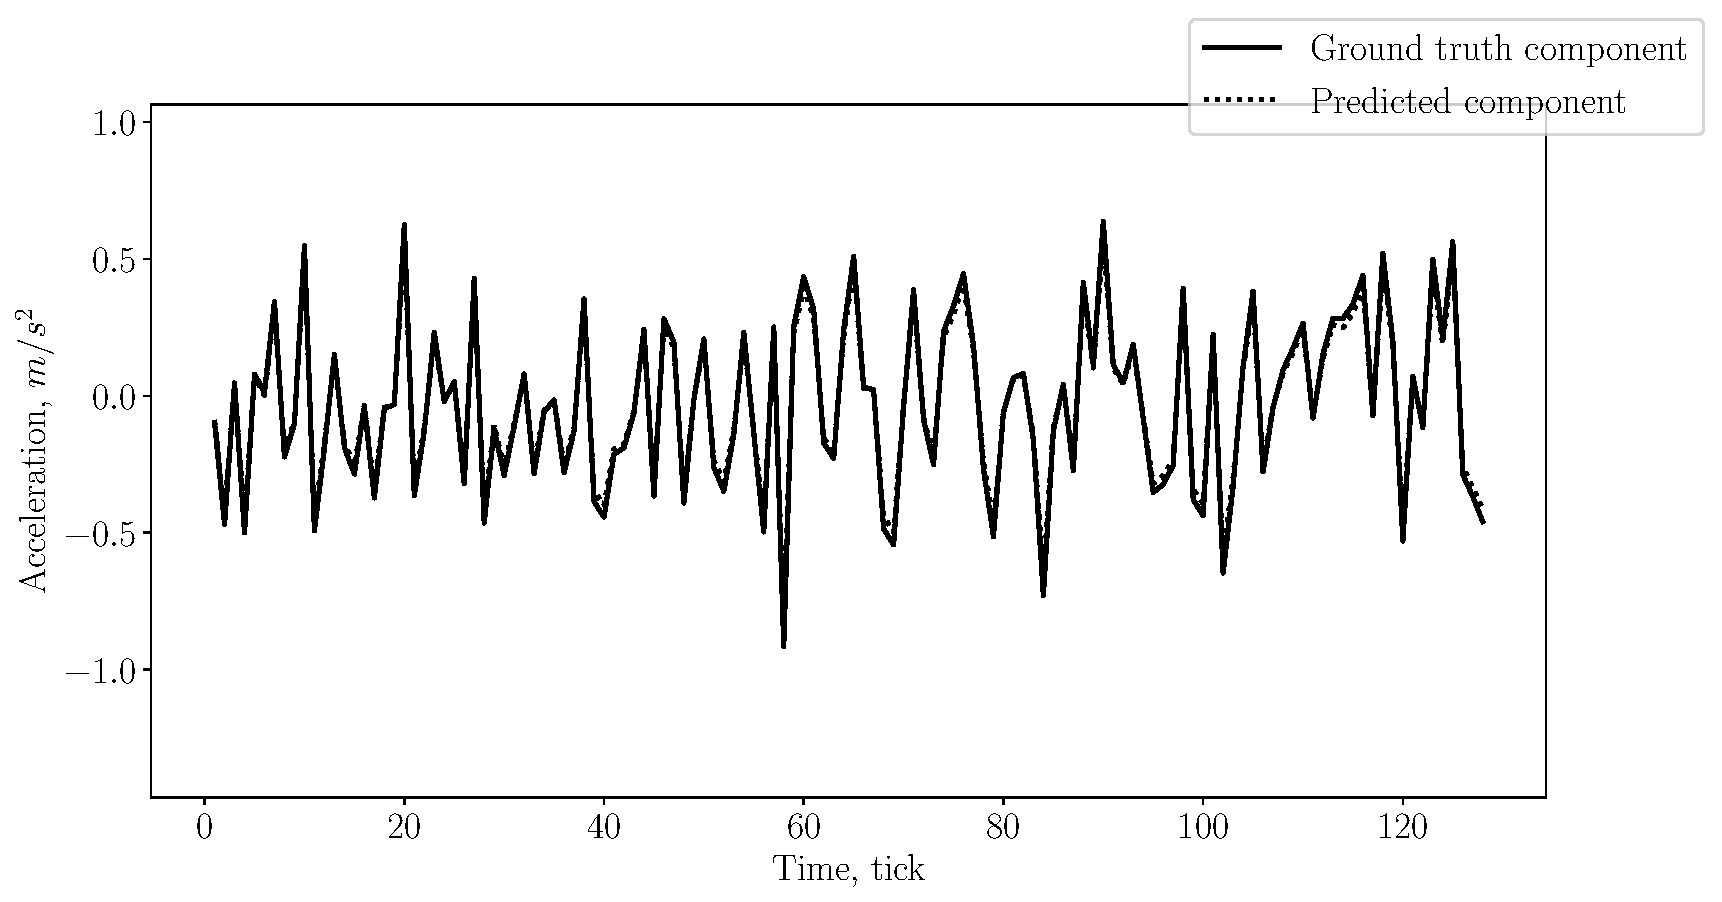
\includegraphics[scale = 0.42]{experiment4_1000.pickle_results_a.pdf}}
 
 \subfloat[]{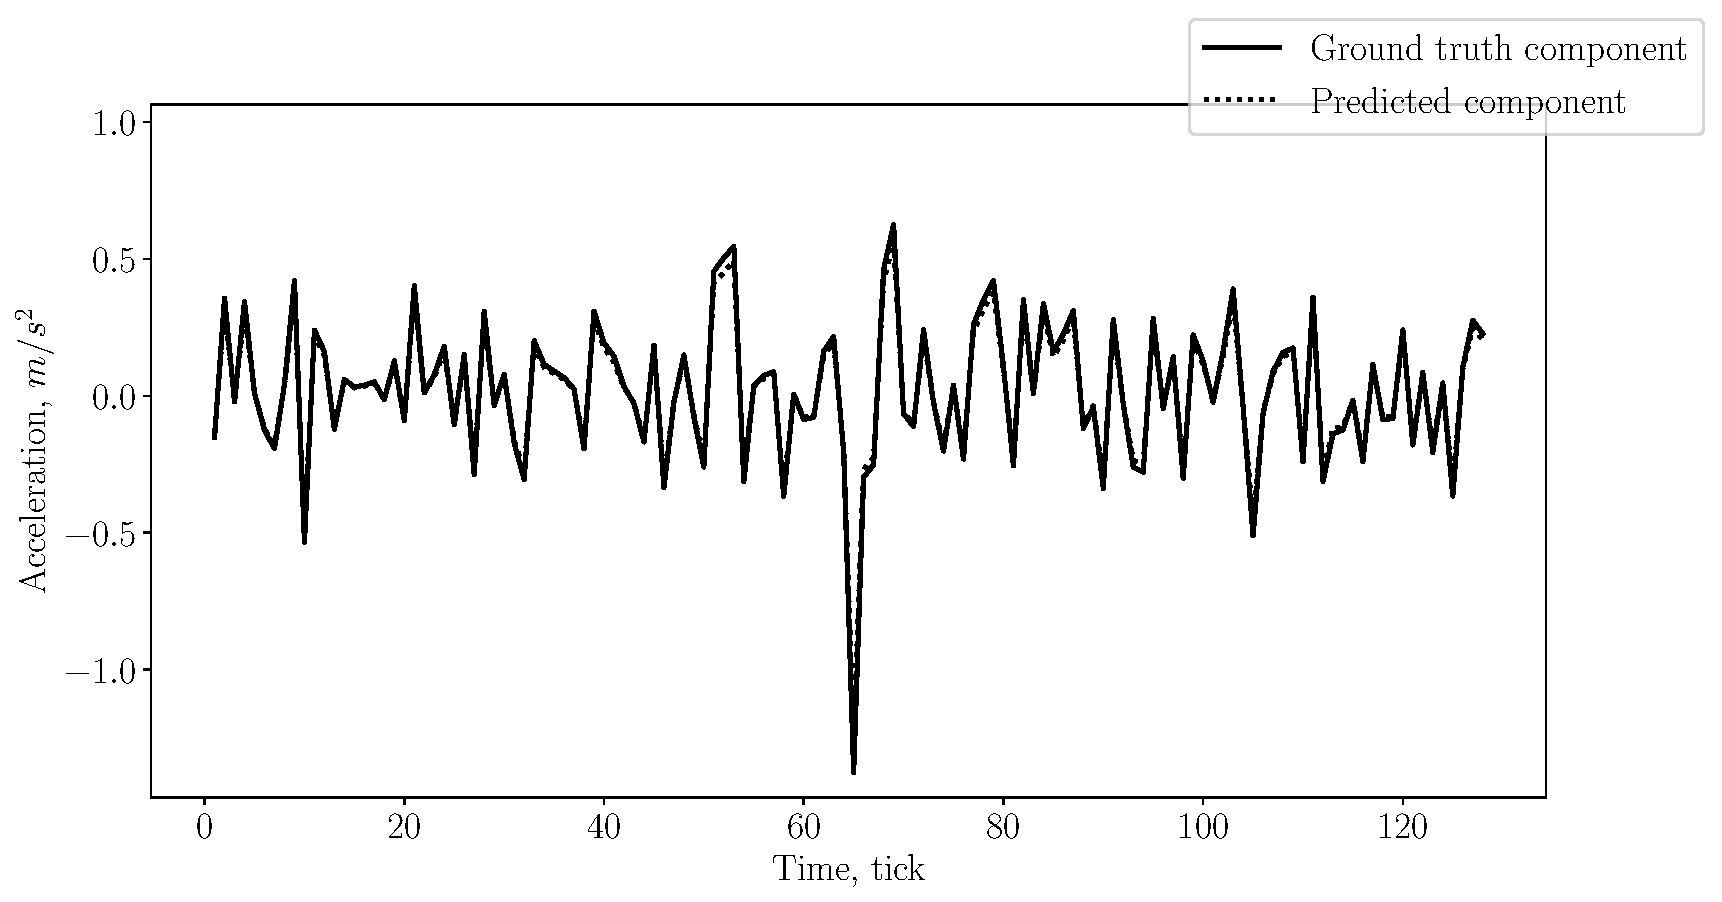
\includegraphics[scale = 0.42]{experiment4_1000.pickle_results_b.pdf}}
 \caption{Временной ряд зависимости ускорения от времени для тестовой выборки (а) реальные данные, (б) предсказанные}
 \label{fig: trajectory}
\end{figure}

\begin{figure}[H]
 \centering
 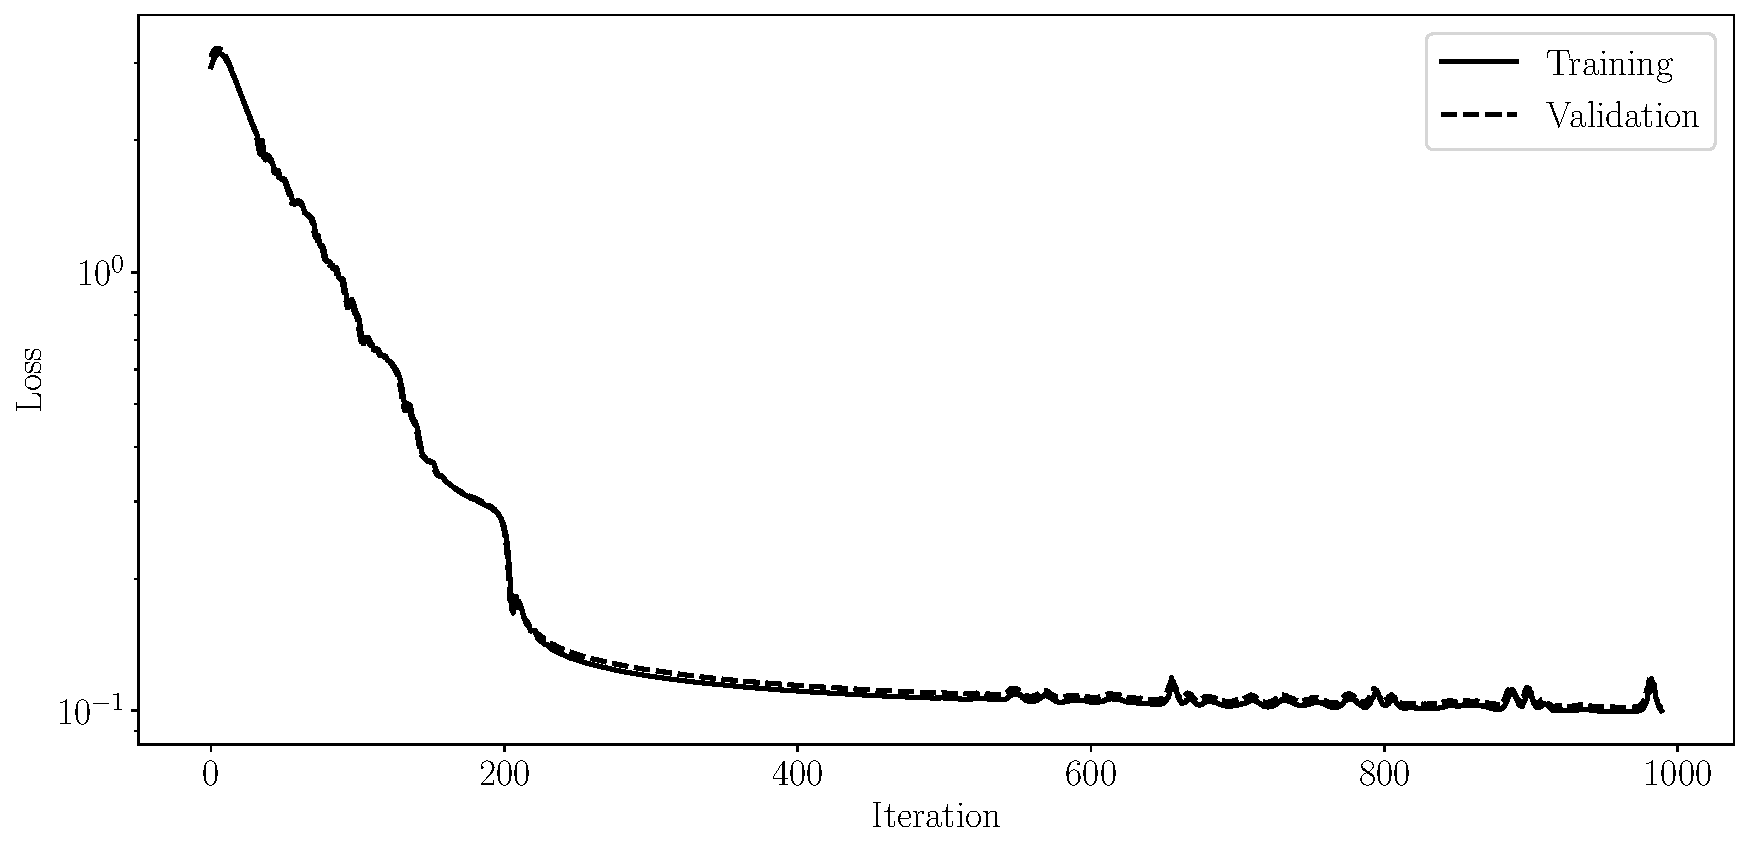
\includegraphics[scale = 0.42]{experiment4_1000.pickle_loss.pdf}
 \caption{Графики обучения модели}
 \label{fig: learning_rate}
\end{figure}

Рисунки \ref{fig: trajectory}, \ref{fig: learning_rate} показывают, что траектории в точности восстанавливаются их лагранжианом, причем мы можем предсказывать их на достаточно большом отрезке времени, потери на тестовой и обучающей выборке близки, а траектории сохраняют свой вид. Это означает, что в соответствие с предположением пространство Лагранжианов является скрытым пространством, из которого сгенерированы все траектории.

Таким образом $\hat{L}_i$ векторизует данные $X_i$ для дальнейшей классификации. В замечании к лемме \ref{lemma2} введена норма на пространстве лагранжианов, что представляет его как гильбертово пространство. Окончательно, векторизации берется из замечания \ref{remark3}, в котором пространство лагранжианов проецируется на евклидово пространство $\mathbb{R}^n$. Векторизация траектории соответствует векторизации их лагранжианов.

В отличие от работы \cite{article} предлагается дополнительно регуляризовать функцию потерь. Т. к. в областях, где собственные числа матрицы$H = \left(\nabla_{\dot{\mathbf{q}}\dot{\mathbf{q}}} L\right)_{i j}=\frac{\partial^{2} L}{\partial \dot{q_{j}} \partial \dot{q}_{i}}.$ стремятся к 0 решение является неустойчивым, а на траекториях выявляются нефизические колебания. Поэтому вводится дополнительный член $\mathcal{L}_\text{restriction} =  \sum \alpha * a(\beta(1 - \lambda(H)_i)$, где $a$ некоторая линейная функция активации, лучше всего себя показала $a = SiLU = x*\sigma(x)$. Гиперпараметры $\alpha, \beta$ настраиваются в зависимости от типа данных, для данного датасета подобраны $\alpha = 5, \beta = 12$

Для полученной оценки лагранжиана можно сэмплировать значения функции в любой точке $(\mathbf{q},\ \mathbf{\dot{q}})$. Соответственно сэмплируется норма, на основе которой строится метрика, а на основе этой метрики уже классифицируются траектории базовыми алгоритмами.

Поэтому для начала получается набор точек, в которых получаются значения лагранжиана. Этот набор получаетсся до классификации, и он един для всех траекторий. Соответственно он является гиперпараметром для классификатора. Получается набор $S = \{s_i\}$ из $N = 20000$ точек $(\mathbf{q},\ \mathbf{\dot{q}})$ равномерно распределенных на кубе $-10 \le {x_i} \le 10$. Размер куба подбирается так, чтобы он покрывал точки, на которых обучаются лагранжианы. Число точек для сэмплирования должно быть подобрано так, чтобы оценка нормы менялась слабо по сравнению с ее оценкой.

Для каждого объекта получаются значения $X_i = \{AL(s_i)\}$ набор его признаков. Норма в этом пространстве соответствует обычной евклидовой норме, а для классификации объектов в данном пространстве используются базовые алгоритмы классификации веторов. Классифицировать объекты предлагается по их признакам, т. е. сэмплированным значениям нормы.

\[A(L)\ =\ \frac{\partial L}{\partial \mathbf{q}}-\frac{\partial}{\partial \mathbf{q}} \frac{\partial L}{\partial \dot{\mathbf{q}}} \dot{\mathbf{q}}\]

Для регуляризации и уменьшения размерности применим метод главных векторов для преобразования признаков. После этого для исследования набора представим объекты по первым трем главным признакам на 2D и 3D-графиках.

\begin{figure}[H]
 \centering
 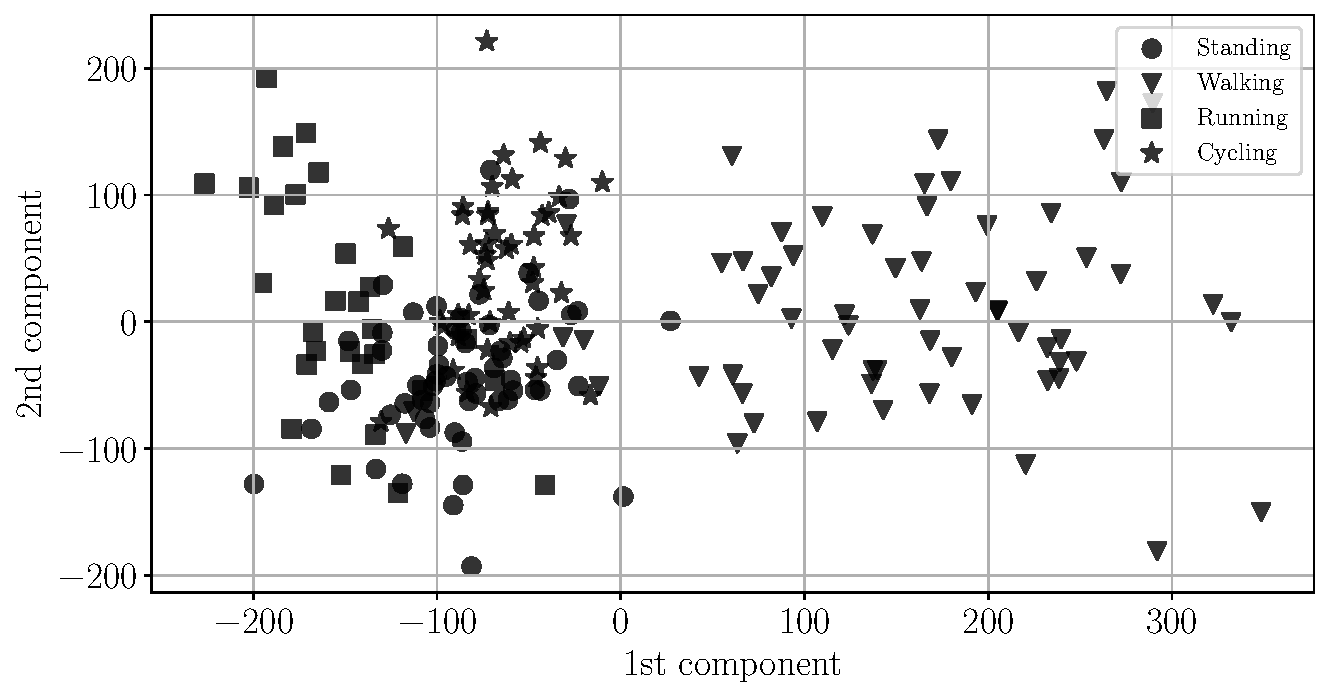
\includegraphics[scale = 0.5]{Data.pdf}
 \caption{Проекция оценок лагранжианов $\hat{L}$ на 2D-поверхность}
 \label{fig: 2D}
\end{figure}

\begin{figure}[H]
 \centering
 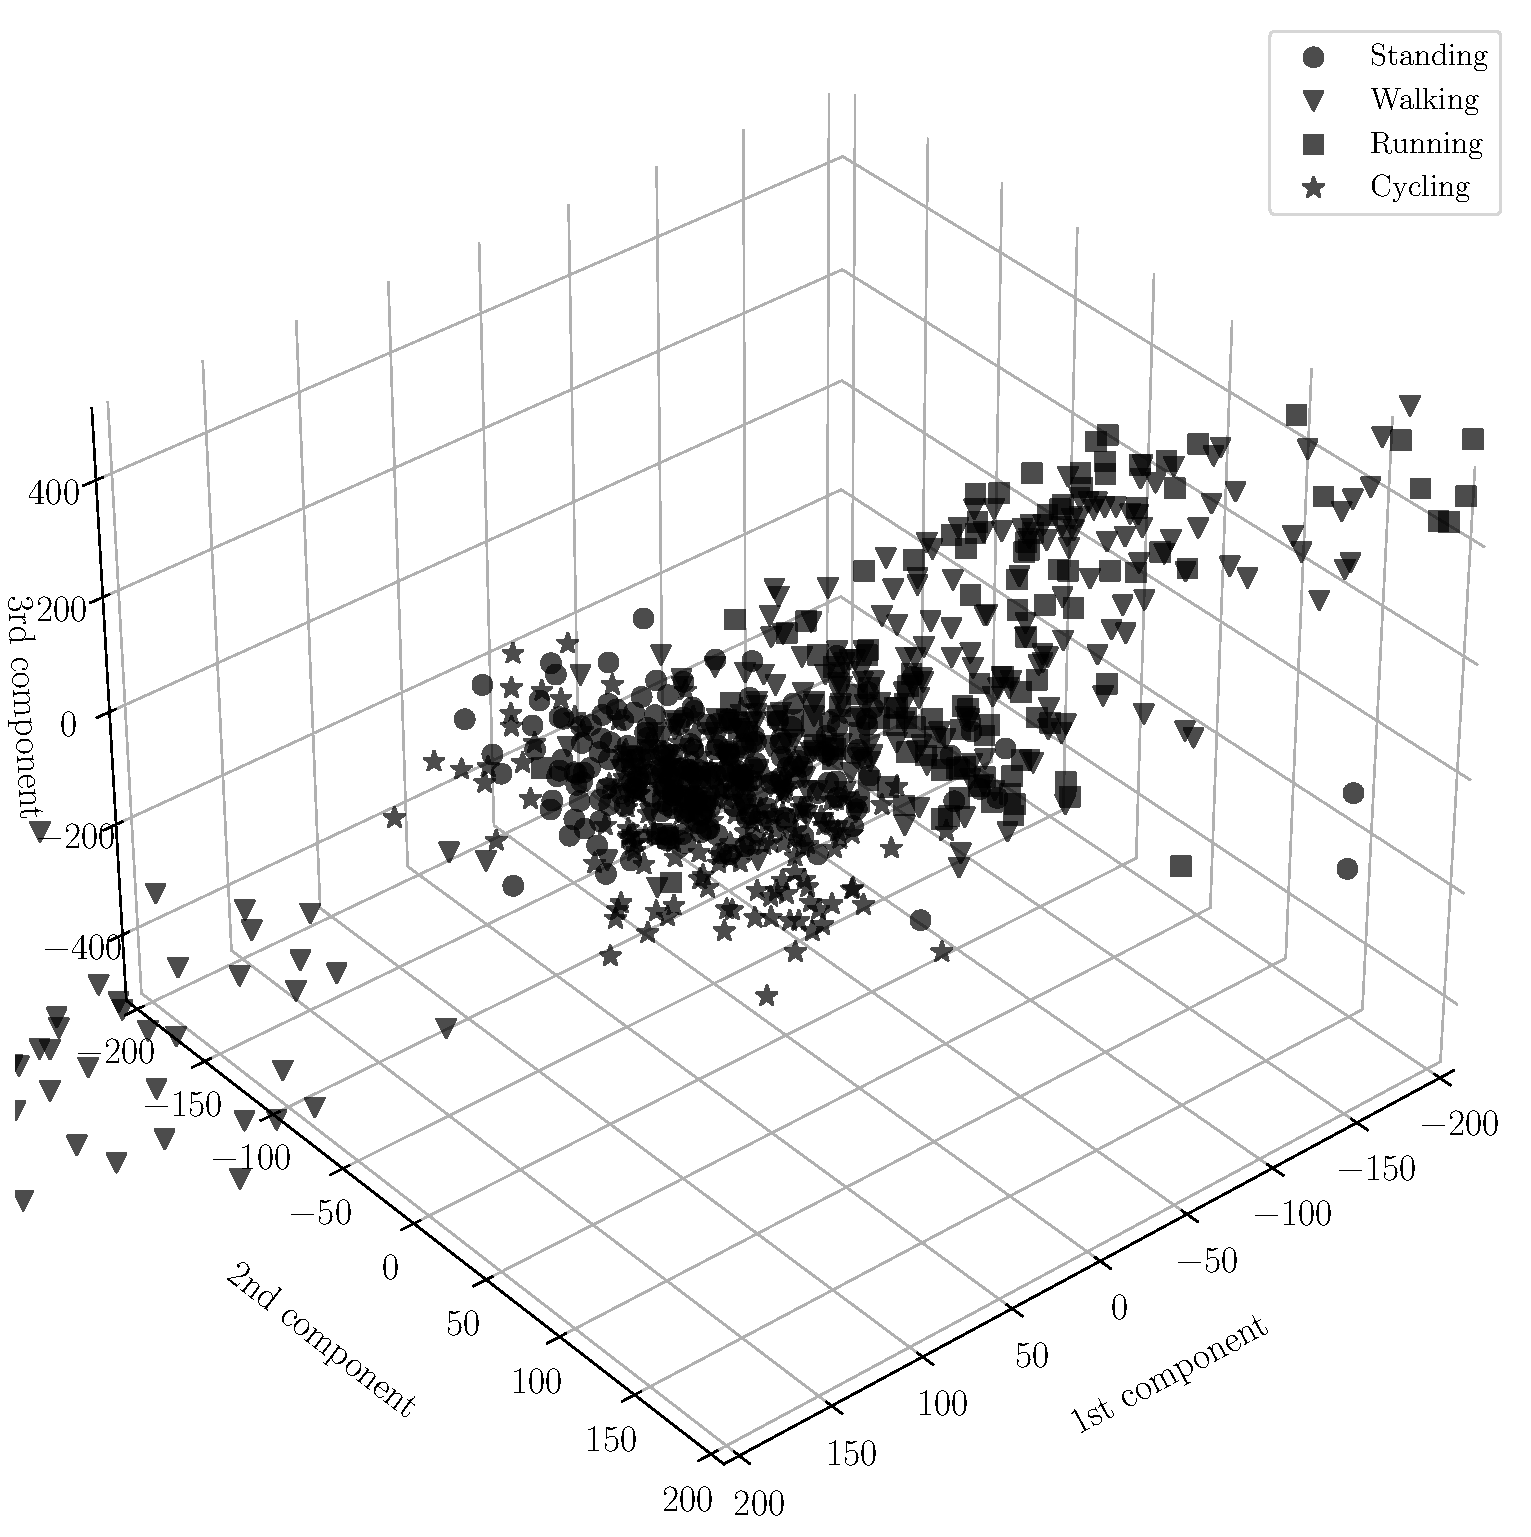
\includegraphics[scale = 0.4]{Data_3D.pdf}
 \caption{Проекция оценок лагранжианов $\hat{L}$ на 3D-поверхность}
 \label{fig: 3D}
\end{figure}

Из графиков \ref{fig: 2D}, \ref{fig: 3D} следует, что данные разделяются на различные кластеры, распределенные по нормальному закону, и предполагается, что они разделяются метрическими методами с гауссовским ядром. Из графиков следует то, что в представленное пространство лагранжианов классы отделяются линейными поверхностями и следует использовать линейные модели для дальнейшей классификации.
\newpage
\paragraph{Исследование моделей.}Для исследования был выбор случайный лес, т.к. он хорошо работает с любыми сложными наборами данных, линейная регрессия и гауссовский процесс, как достаточно простые классификаторы которые быстро учатся и соответственно полезно знать работают ли они на наборе данных, а также SVC с гауссовским ядром, т.к. по визуальному анализу предполагается, что данные распределены по нормальному закону.


\begin{figure}[H]
 \centering
 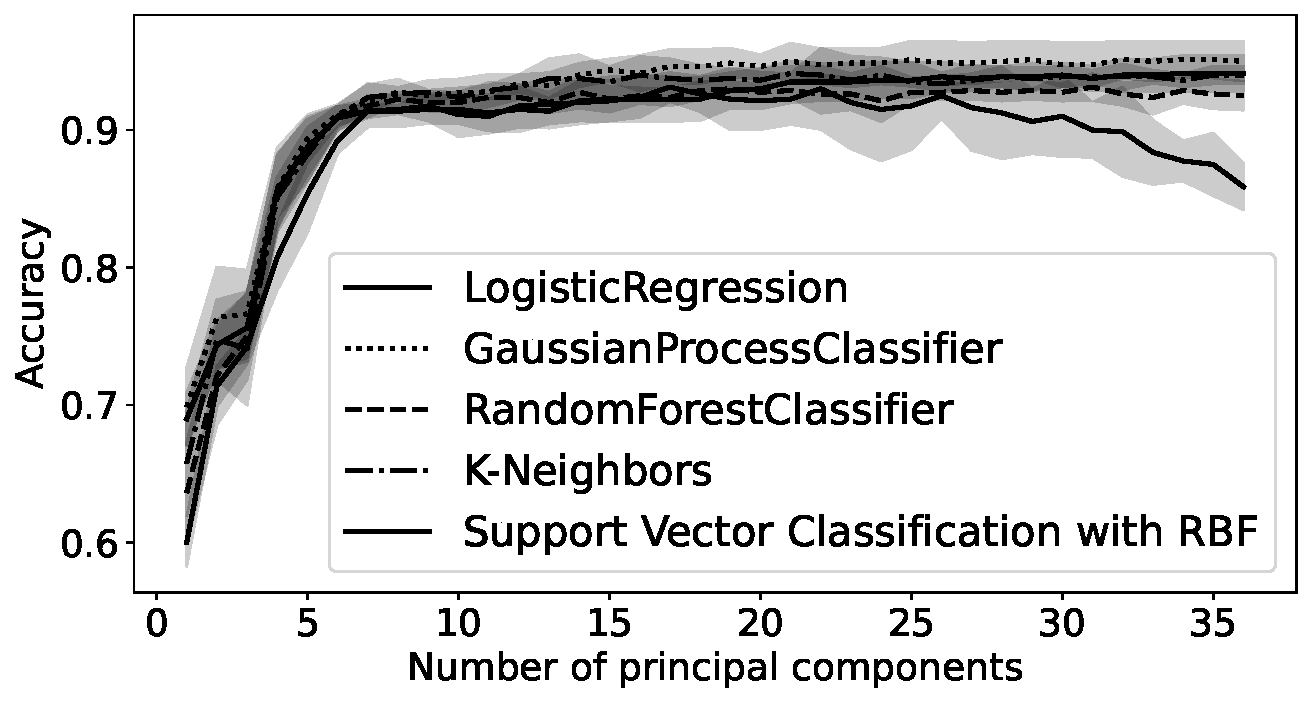
\includegraphics[scale = 0.7]{Accuracy.pdf}
 \caption{Точность классификации выбранных методов в зависимости от числа главных компонент}
 \label{fig: Accuracy}
\end{figure}


\begin{table}[H]
    \centering
    \begin{tabular}{|l|lll|}
    \hline
    \multicolumn{1}{|c|}{\multirow{2}{*}{Классификатор}} & \multicolumn{3}{c|}{Метрика}                                                                     \\ \cline{2-4} 
    \multicolumn{1}{|c|}{}                               & \multicolumn{1}{l|}{Accuracy}         & \multicolumn{1}{l|}{Balanced-accuracy} & F1 Macro        \\ \hline
    Логистическая регрессия                              & \multicolumn{1}{l|}{$0,927 \pm  0.014$} & \multicolumn{1}{l|}{$0,924 \pm 0,13$}    & $0,927 \pm 0,14$  \\ \hline
    \textbf{Гауссовский процесс}                                  & \multicolumn{1}{l|}{$\mathbf{0,946} \pm \mathbf{0,010}$}  & \multicolumn{1}{l|}{$\mathbf{0,941} \pm \mathbf{0,011}$}   & $\mathbf{0,946} \pm \mathbf{0,010}$ \\ \hline
    Случайный лес                                        & \multicolumn{1}{l|}{$0,932 \pm 0,007$}  & \multicolumn{1}{l|}{$0,928 \pm 0,008$}   & $0,933 \pm 0,008$ \\ \hline
    K-ближайших соседей                                  & \multicolumn{1}{l|}{$0,939 \pm 0,009$}  & \multicolumn{1}{l|}{$0,935 \pm 0,010$}   & $0,940 \pm 0,008$ \\ \hline
    SVC с гауссовским ядром                              & \multicolumn{1}{l|}{$0,933 \pm 0,012$}  & \multicolumn{1}{l|}{$0,927 \pm 0,01$3}   & $0,933 \pm 0,011$ \\ \hline
    \end{tabular}
    \caption{Результат работ классификаторов на предложенной векторизации данных}
    \label{table:classifictors}
\end{table}

Стабильнее всего обучается SVC, на нем отсутствует переобучение, и он показывает результаты сравнимые с остальными классификаторами, гауссовская переобучается, поэтому абсолютно не подходит под модель. Гауссовский процесс и логистическая регрессия на пространстве больших размерностей. remark Случайный лес работает на уровне SVC

\paragraph{Сравнение с другими классификаторами}
Также были проведены сравнения с существующими методами классификации временных рядов. Метод случайного леса для временных рядов TimeSeriesForestClassifier, приставленный в библиотеке Sktime показывает на том же наборе данных точность в 78\%, что намного хуже LNN-классификатора

\newpage
\section{Заключение}

Представление траектории в виде лагранжианов физических систем, которым они соответствуют, предложенное в ранних работах, является мощным инструментом для классификации траекторий. Данный метод имеет множество преимуществ по сравнению с методами классификации, не использующие информацию о физике системы. Метод является многомерным уже по своей природе, нам не нужно вводить никаких предположений о связи между различными компонентами траекторий. Он устойчив к изменениям данных, сохраняющих физику системы. Предложенная векторизация данных сохраняет физические предположения о близости данных. В том числе метод дает удобный способ для проецирования данных на плоскость для дальнейшей визуализации. Визуальный анализ графиков показывает, что представленное пространство лагранжианов соответствует пространству признаков, которые задают класс траекторий, т.е. они определяют вид движения. Аналогичные результаты показывает обучение линейных моделей на данном векторном пространстве, из графиков следует, что с точностью 0.95 линейные модели разделяют классы, представленные в наборе данных.  В то же время предложенная векторизация затратна по времени, а также требуется настройка параметров регуляризации для достижения необходимой точности аппроксимации на конкретных наборах траекторий

\newpage

\begin{thebibliography}{99}
\bibitem{PINNreview}
    \BibAuthor{Karniadakis, G.E., Kevrekidis, I.G., Lu, L. et al.} Physics-informed machine learning ~// \BibJournal{Nat Rev Phys 3}, 422–440 (2021). \BibDoi{10.1038/s42254-021-00314-5}
\bibitem{LGNN}
    \BibAuthor{Ravinder Bhattoo et al.} Learning the dynamics of particle-based systems with Lagrangian graph neural networks ~// \BibJournal{Mach. Learn.: Sci. Technol. 4 015003} (2023). \BibDoi{10.1088/2632-2153/acb03e}
\bibitem{Fluid-LNN}
    \BibAuthor{Henning Wessels, Christian Weißenfels, Peter Wriggers} The neural particle method – An updated Lagrangian physics informed neural network for computational fluid dynamics ~// \BibJournal{Computer Methods in Applied Mechanics and Engineering, Vol. 368} (2020), 113127. \BibDoi{10.1016/j.cma.2020.113127}
\bibitem{Deconstruct-HNN}
    \BibAuthor{Nate Gruver, Marc Finzi, Samuel Stanton, Andrew Gordon Wilson} Deconstructing the Inductive Biases of Hamiltonian Neural Networks ~// \BibJournal{ ICLR} (2022), \BibDoi{10.48550/arXiv.2202.04836}
\bibitem{MTCSreview}
    \BibAuthor{Ruiz AP, Flynn M, Large J, Middlehurst M, Bagnall A.}
    The great multivariate time series classification bake off: a review and experimental evaluation of recent algorithmic advances. ~// \BibJournal{Data Min Knowl Discov.} (2021),
    \BibDoi{10.1007/s10618-020-00727-3}
\bibitem{MTCSindustrial}
    Multivariate Time-Series Classification of Critical Events from Industrial Drying Hopper Operations: A Deep Learning Approach
\bibitem{MTCSactivity}
    \BibAuthor{S. Seto, W. Zhang and Y. Zhou}
    Multivariate Time Series Classification Using Dynamic Time Warping Template Selection for Human Activity Recognition
    ~// \BibJournal{IEEE Symposium Series on Computational Intelligence} pp. 1399-1406 (2015), \BibDoi{10.1109/SSCI.2015.199}
\bibitem{article}
 \BibAuthor{M. Cranmer, S. Greydanus, S. Hoyer et al. }
 Lagrangian neural networks~//
 \BibJournal{ICLR 2020 Deep Differential Equations Workshop}.
	\BibDoi{10.48550/arXiv.2003.04630}.
\bibitem{TCSreview}
    \BibAuthor{Ismail Fawaz, H., Forestier, G., Weber, J. et al.} Deep learning for time series classification: a review~// \BibJournal{Data Min Knowl, Disc 33, 917–963 (2019)} \BibDoi{10.1007/s10618-019-00619-1}
\bibitem{ROCKET}
    \BibAuthor{Dempster A, Petitjean F, Webb G}
    ROCKET: exceptionally fast and accurate time series classification using random convolutional kernels.
    \BibJournal{Data Min Knowl Disc 34 1454–1495 (2020)} \BibDoi{10.1007/s10618-020-00701-z} 
\bibitem{HNNreduce}
    \BibAuthor{Dempster A, Petitjean F, Webb G}
    Canonical and noncanonical Hamiltonian operator inference
    \BibJournal{Computer Methods in Applied Mechanics and Engineering, Vol. 416 (2023)} \BibDoi{10.1016/j.cma.2023.116334} 
\bibitem{HNNadapt}
    \BibAuthor{Dempster A, Petitjean F, Webb G}
    Adaptable Hamiltonian neural networks
    \BibJournal{Phys. Rev. Res.} Vol. 3 (2021) \BibDoi{10.1103/PhysRevResearch.3.023156} 
\bibitem{HNNrobustclass}
    \BibAuthor{Zakwan Muhammad, Xu Liang,  ferrari trecate Giancarlo.}
    Robust Classification Using Contractive Hamiltonian Neural ODEs
    \BibJournal{IEEE Control Systems Letters}.  7. 145-150. (2021) \BibDoi{10.1109/LCSYS.2022.3186959} 
\bibitem{PINNsoundwave}
    Physics-Informed Neural Network for Volumetric Sound field Reconstruction of Speech Signals
\bibitem{HNN}
    \BibAuthor{Samuel Greydanus, Misko Dzamba, Jason Yosinski}
    Hamiltonian Neural Networks
\bibitem{quantumHNN}
    \BibAuthor{Kris Tucker, Amit Kiran Rege, Conor Smith, Claire Monteleoni, Tameem Albash}
    Hamiltonian Learning using Machine Learning Models Trained with Continuous Measurements
\end{thebibliography}

%%%% если имеется doi цитируемого источника, необходимо его указать, см. пример в \bibitem{article}
%%%% DOI публикации, зарегистрированной в системе Crossref, можно получить по адресу http://www.crossref.org/guestquery/
\end{document}
